% !TEX root =  ../../master.tex
\section{Client}
\label{sec:ClientImplementierung}

% !TeX root = ../../../master.tex

\subsection{Geschäftslogik}
\label{ssec:GeschaeftslogikClient}

In diesem Projekt soll React zum Einsatz kommen, welches bereits im Grundlagenteil kurz beschrieben wurde (Kapitel~\vref{ssec:React}).
Durch die Verwendung von React wird keine hardware-spezifische Software benötigt.
Die Anwendung kann sowohl als Webanwendung als auch auf einem mobilen Gerät benutzt werden.
Dadurch wird Anforderung der endgeräteunabhängigen Nutzung (\hyperref[Anf:A1]{A1}) erfüllt.
React wurde \ua deshalb für die Entwicklung des Front-Ends ausgewählt, da es seit mehreren Jahren kontinuierlich als die beliebteste Front-End-Bibliothek gilt\autocite[Vgl.][]{stackoverflow_Top_Frameworks} und zudem verhältnismäßig leicht zu erlernen ist.
Darüber hinaus werden Komponenten verwendet, die als modulare Grundlage dienen und ein wiederholtes Schreiben des Codes verhindern sollen (Boilerplate-Code).


Für die Unterteilung der verschiedenen Komponenten wurde der Wert besonders auf eine angenehme \acf{UX} und ein benutzerfreundliches \acf{UI} gelegt.
Da die Anwendung im Rahmen eines Projektes der \acs{DHBW} Mannheim konzeptioniert wird, sollen die Komponenten gemäß Anforderung~\hyperref[Anf:A16]{A16} das entsprechende Farbschema nutzen (vgl. Kapitel~\vref{sec:konzeption:client}).
Im folgenden wird auf den Aufbau der Benutzeroberfläche (\ac{UI}) des Clients eingegangen.


% !TeX root = ../../../master.tex

\subsection{Aufbau React}
\label{ssec:AufbauReact}

Um React bzw. den Komponentenaufbau zu verstehen, ist es nötig zu wissen, wie die Komponenten miteinander interagieren. 
Hierzu zählt \ua das Verständnis, dass eine Komponente Parameter von ihrerer Elternkomponente übermittelt bekommen kann (\props). 
Wie auch in anderen Programmiersprachen wie \zb Java, wird ein Konstruktor \engl{constructor} zur Instanziierung einer Komponente verwendet.
Dieser erlaubt den Zugriff auf die übermittelten \props. 

Die Hauptmethode zum Anzeigen einer Komponente im \ac{UI} ist die \render-Funktion. 
In ihr wird das Aussehen der Komponente definiert, welches deskriptiv über \acs{HTML} oder weitere Kind-Kompo\-nente(n) beschrieben wird. 
Wichtig zu verstehen ist hierbei, dass beim Laden einer solchen Komponente der in React definierte Lebenszyklus duchlaufen wird (siehe Abb. \ref{fig:ReactLifecylce}).
Für die Umsetzung dieses Projektes sind die nachfolgend beschriebenen Zustände (Methoden) des Lebenszykluses besonders wichtig. 
Zum einen wird beim Laden die Funktion \cwm aufgerufen, die Änderungen vor dem kompletten Laden der Komponente vollzieht.
Dies sollte jedoch ab der Version 17 nicht mehr verwendet werden. 
Zum zweiten wird nach dem Erstellen der Komponente die Funktion \cdm aufgerufen. 
Diese ermöglicht es \zb den \state  der Anwendung zu verändern. 
Ein Beispiel hierfür wäre ein Formularfeld, welches den Vor-, Nachname und Alter eines Studenten aus den \props erhält. 
Diese Änderungen erfolgt lediglich auf der zu änderten Komponente über den virtuellen \ac{DOM}. 
Das Ändern des \state wird über eine Funktion \exampleState durchgeführt, welches die neuen Parameter in der Komponente setzt.
Dadurch, dass React nur die Teile bzw. Komponenten ändert, an denen Änderungen aufgetreten sind, wird zudem eine erhöhte Performance im Bezug auf Ladegeschwindigkeit erreicht, da nicht die komplette Seite neu gerendert wird. 

\begin{figure}[ht]
	\centering
	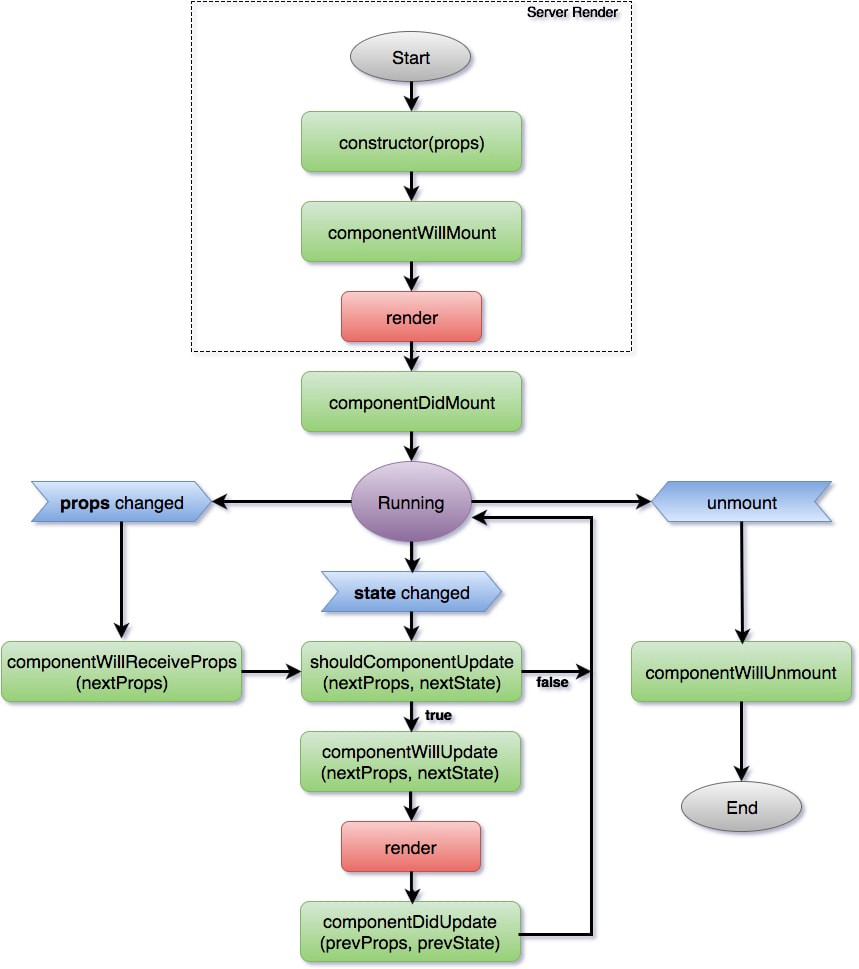
\includegraphics[height=0.60\textheight, keepaspectratio]{img/client/Lifecycle.jpeg}
	\captionsetup{justification=centering, format=plain}
	\caption[Der Lebenszyklus von React]{Der Lebenszyklus von React \\ \quelle \cite{reactLifeCycle}}
	\label{fig:ReactLifecylce}
\end{figure}


% !TeX root = ../../../master.tex

\subsection{Ordnerstruktur}
\label{ssec:Ordnerstruktur}

Wie bereits in den Kapiteln \myRefGeneral{ssec:React} und \myRefGeneral{ssec:AufbauReact} dargelegt, werden für den Aufbau der Anwendung verschiedene Komponenten benötigt. 

Abb. \myRefGeneral{fig:OrdnerstrukturVSCode} zeigt einen Ausschnitt der Ordnerstruktur in der Entwicklungsumgebung \emph{Visual Studio Code (VS Code)}.\footnote{\url{https://code.visualstudio.com}}
Exemplarisch werden kurz die Card-Komponente sowie die Admin-Komponente erläutert, deren Ergebnisse später in Kapiteln A, B, aufgezeigt werden. \todo[]{Ref Chapter}

Für jede Komponente wird in VS Code ein eigener Ordner angelegt, der die Komponente selbst (wie z.B. \jinline|Admin| oder \jinline|Card|) sowie die Kind-Komponenten (wie z.B. \jinline|CreateUserCard|) enthält.  
Des weitern wird eine spezifische \emph{\acs{CSS}}-Datei angelgt, die Anpassungen an den \acsu*{HTML}-Dateien vollzieht. 
Dies könnte z.B. die Farbe in \enquote{DHBW-rot} sein. 
Damit einhergehend kann eine differenzierterer und übersichtlicher Code erzeugt werden. 

Wie bereits beschrieben kann eine Komponente mehrere Kind-Komponenten und diese ebenfalls wieder mehrere Kind-Komponenten enthalten. 
So fungiert die Klasse \jinline|Card| u.a. als Kind-Komponente der Komponente \jinline|CreateUserCard|, \jinline|RegisterKeyCard| und \jinline|ShowUsersCard|. 

\begin{figure}[!htb]
	\centering
	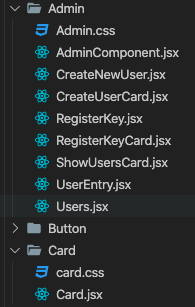
\includegraphics[height=0.4\textwidth, keepaspectratio]{img/client/ordnerStruktur.png}
	\captionsetup{justification=centering, format=plain}
	\caption[Ordnerstruktur in Visual Studio Code]{Ordnerstruktur in Visual Studio Code \\ \quelleScreenshot}
	\label{fig:OrdnerstrukturVSCode}
\end{figure}


\subsection{Participate}
Im Bezug auf Verwendbarkeit wie in Kap. \myRefGeneral{sec:UserJourney} beschrieben ist, soll die Startseite die \emph{Participate}-Seite sein. 
In dieser soll der Benutzer bzw. Student der an einer Umfrage teilnimmt, einen \emph{Surveycode} wie z.B. \emph{\texttt{OYZQGGXOF9}} eingeben, um an der Umfrage zu partizipieren. 

Anschließend wird der Benutzer auf die Umfrageseite weitergeleitet, auf der er die benötigten Felder ausfüllt (siehe Kap. \vref{ssec:UmfrageImplement}).

\begin{figure}[hp]
	\centering
	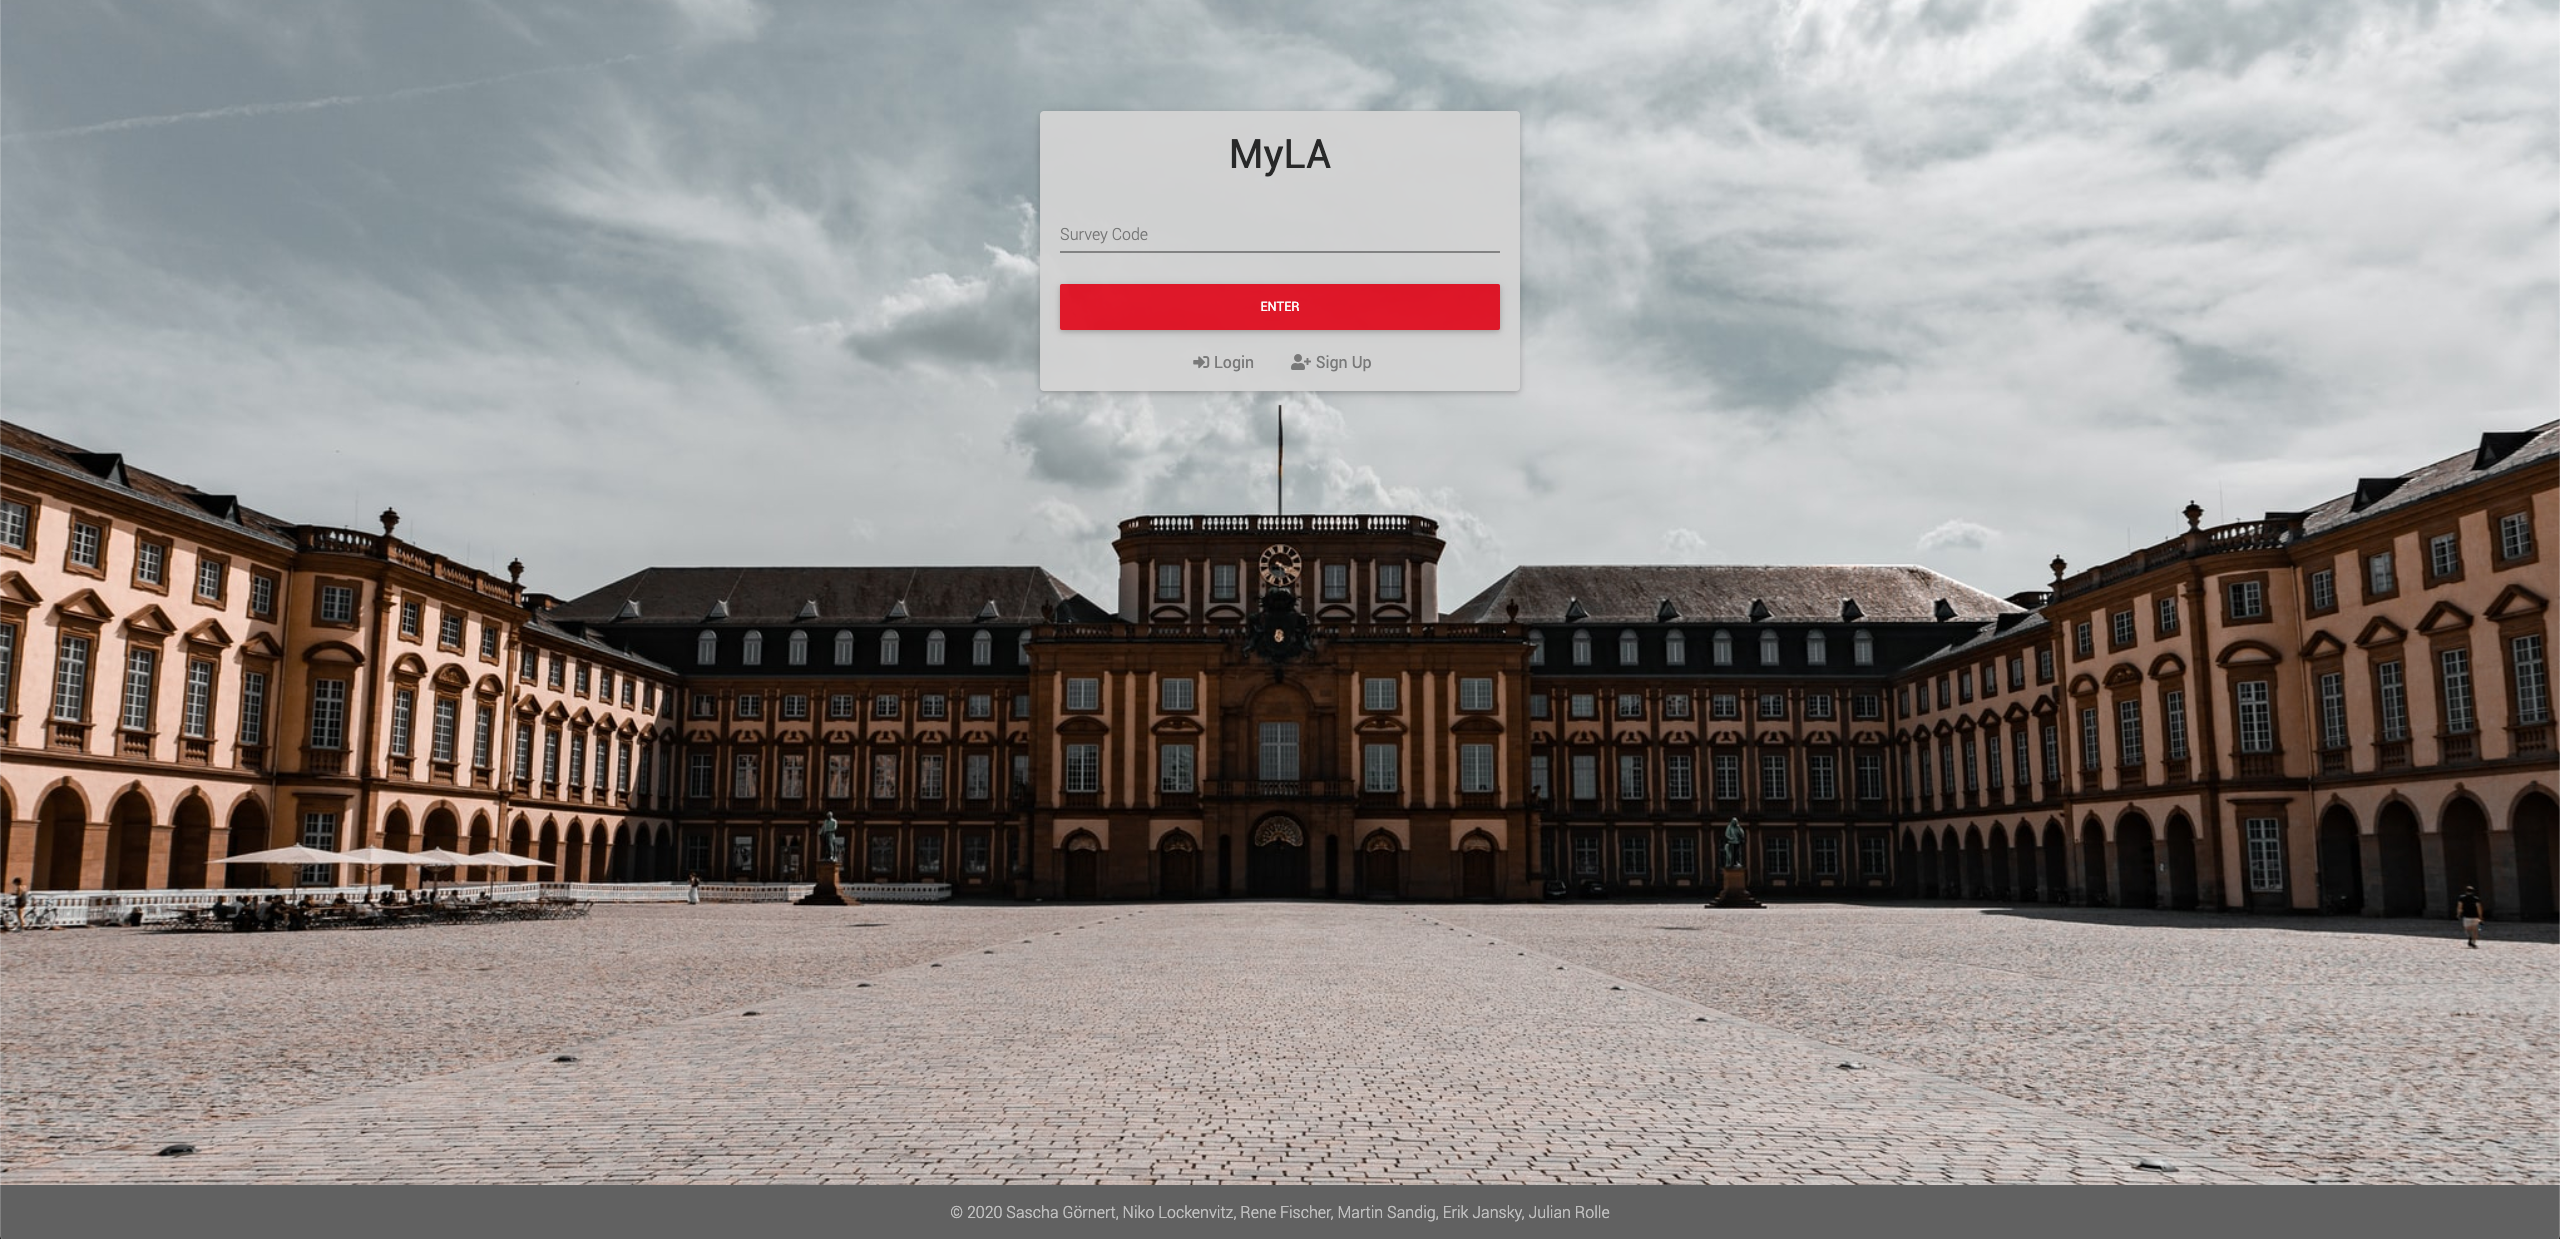
\includegraphics[width=0.95\textwidth, keepaspectratio]{img/client/Participate.png}
	\captionsetup{justification=centering, format=plain}
	\caption[\acf{UI}: Teilnahme Umfrage]{\acf{UI}: Teilnahme Umfrage \\ \quelleScreenshot}
	\label{fig:ParticipateImplement}
\end{figure}

\subsection{Umfrage}
\label{ssec:konzept:client:umfrage}
Wie in Abbildung~\vref{fig:MockUmfrageTeilnehmer} dargestellt, wird der Teilnehmer auf die zuvor angegebene Umfrage geleitet.
Die Fragen werden dabei jeweils in einer eigenen Karte dargestellt.
Durch Drücken eines Knopfes soll der Teilnehmer zur nächsten Frage gelangen.
Gleichzeitig soll dem Benutzer sein Fortschritt verdeutlicht werden, um die Dauer der Umfrage abschätzen zu können.
Die Abgabe der Umfrage erfolgt identisch zum Fragenwechsel.
Der Teilnehmer soll dabei Feedback erhalten, ob seine Teilnahme erfolgreich war.

Durch diesen Vorgang sollen die Anforderungen~\hyperref[Anf:A14]{A14}, die anonyme Teilnahme, sowie \hyperref[Anf:15]{A15}, die einfache Teilnahme an einer Umfrage, erfüllt werden.

\begin{figure}[H]
	\centering
	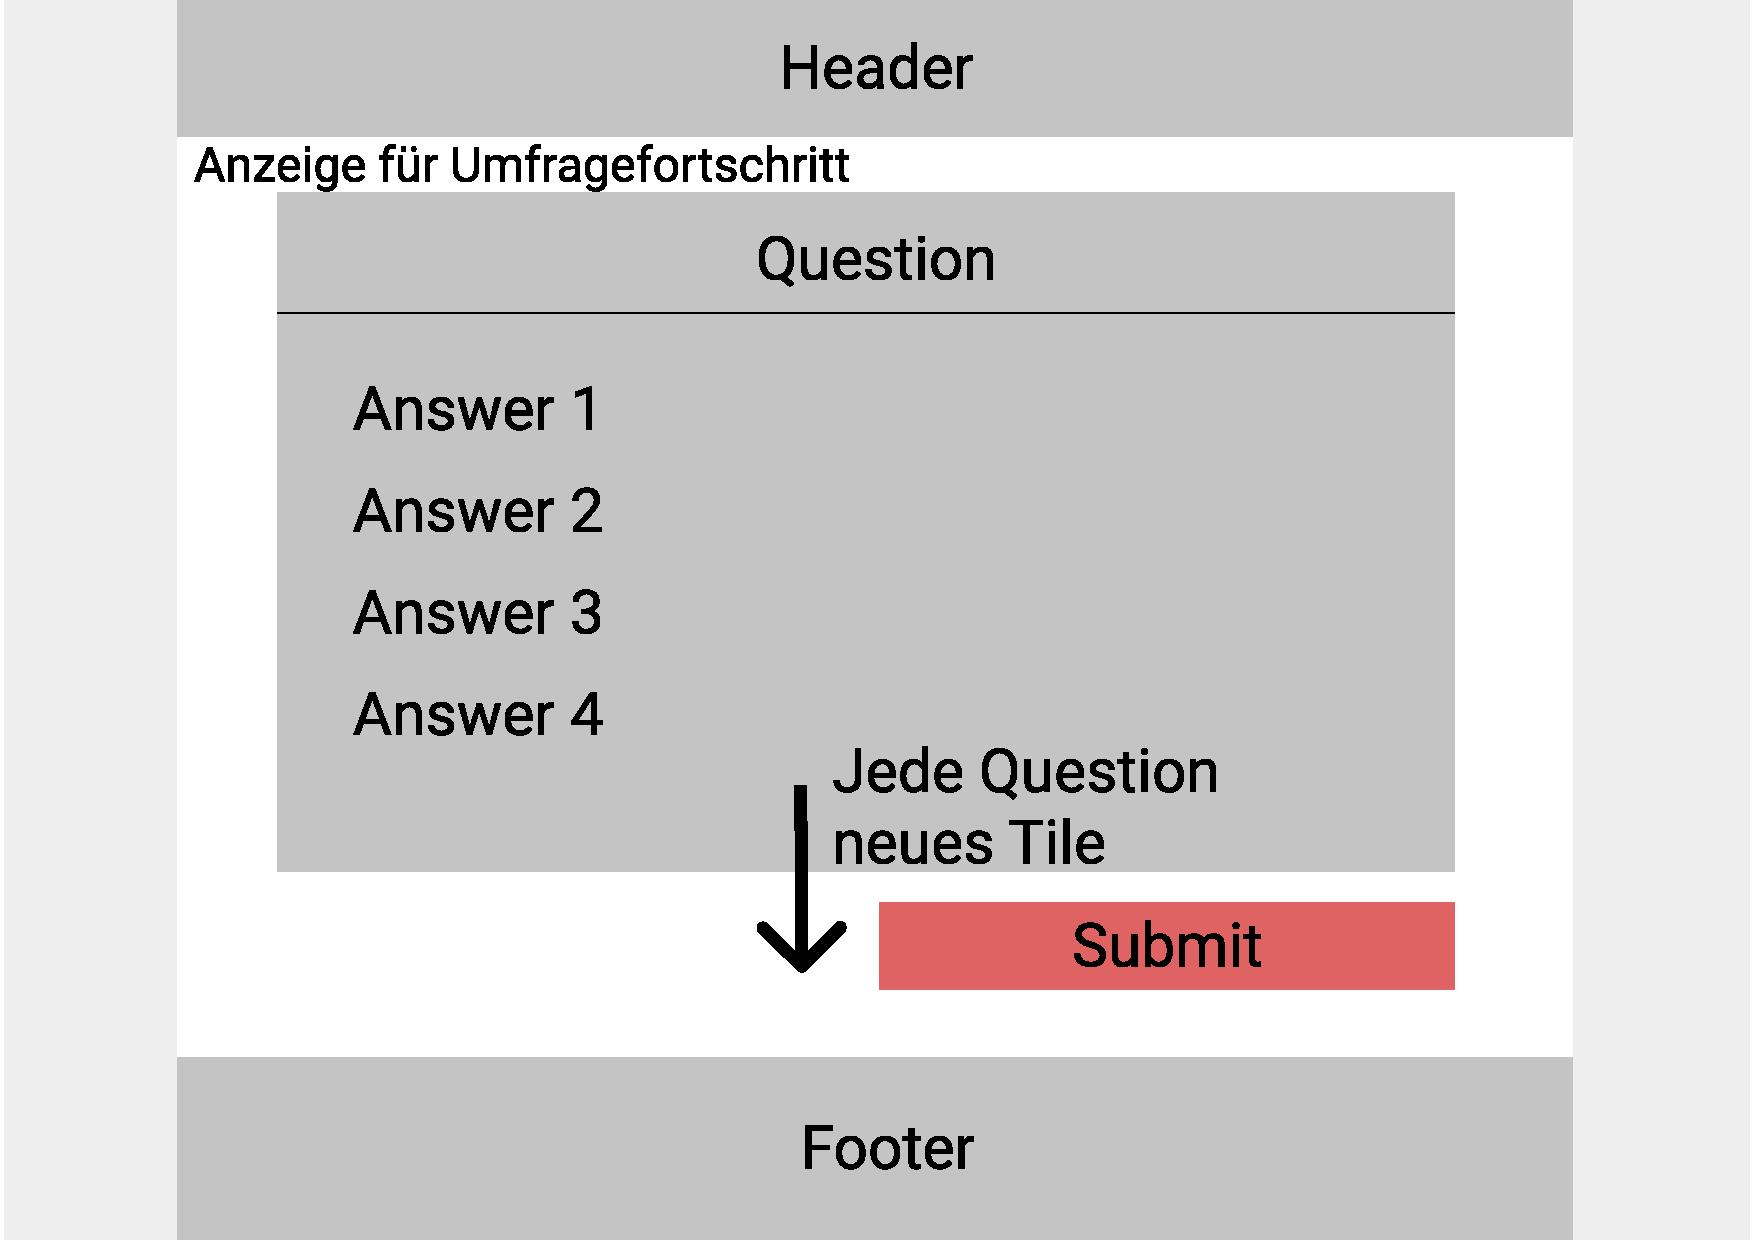
\includegraphics[width=0.7\textwidth]{img/konzeption/client/umfrage_teilnehmer}
	\captionsetup{justification=centering, format=plain}
	\caption[Mock-Up der Teilnahmeseite]{Mock-Up der Teilnahmeseite\\\figma}
	\label{fig:MockUmfrageTeilnehmer}
\end{figure}


\subsection{Signup}
\label{ssec:konzept:client:signup}
Um eine Umfrage erstellen zu können, an der Umfrageteilnehmer partizipieren können, muss zuvor ein Nutzerkonto erstellt werden. 
Hierfür wählt der Benutzer wie in Abb. \ref{fig:MockSignup} dargestellt das Formfeld mit seinem Benutzernamen wie \zb \emph{\texttt{Martin}}. 
Danach wird die E-Mail des Benutzers verlangt, um die Person verifizieren zu können. 
Inwiefern die Identifizierung von den Benutzern geschieht, ist zum Zeitpunkt der Erstellung der Mockups noch nicht klar. 
Eine Möglichkeit, worauf sich in diesem Mockup bezogen wird, ist jedoch die Authentifizierung über die E-Mail-Adresse der DHBW. 
Anschließend wählt der Benutzer ein Passwort seiner Wahl. 
Ist das gewählte Passwort konkludent, so wird der Benutzer angelegt.
Durch das wiederholte eingeben des Passwortes wird sichergestellt, dass es zu keiner Verwirrung bezüglich des gesetzten Passwortes kommt. 
Mit der wiederholten Eingabe des Kennwortes, wird der Nutzer bei unkonkludenten Passwörtern mit einer Fehlermeldung darauf hingewiesen.

\begin{figure}[H]
	\centering
	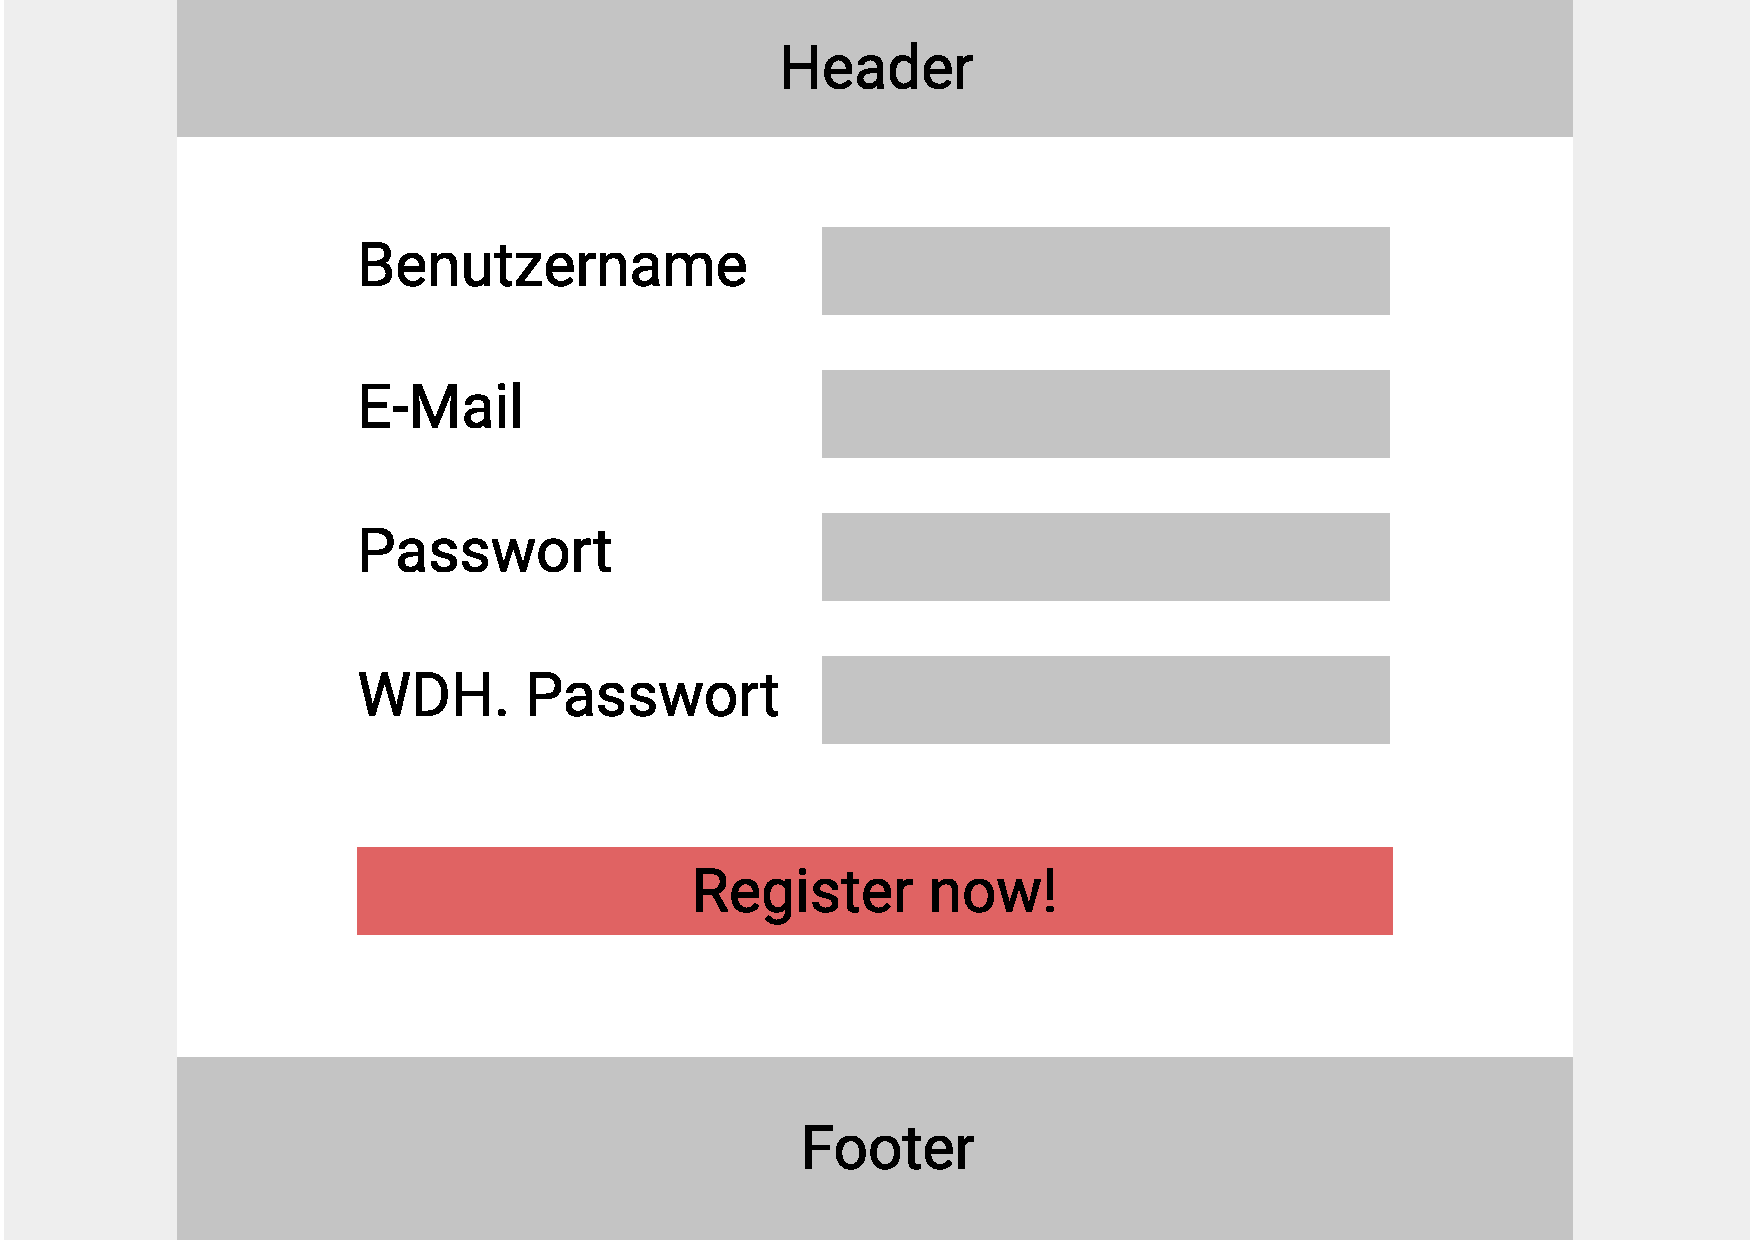
\includegraphics[width=0.7\textwidth]{img/konzeption/client/register}
	\captionsetup{justification=centering, format=plain}
	\caption[Mock-Up der Startseite]{Mock-Up der Registierungsseite \\\figma}
	\label{fig:MockRegister}
\end{figure}

\subsection{Result-Dashboard}
\label{ssec:konzept:client:dashboard}

Das Dashboard soll die Kernkomponente dieser Anwendung sein. 
Auf dieser sollen sämtliche Umfragen und deren Ergebnisse dargestellt werden, wie es in Abbildung \ref{MockDashboard} zu sehen ist.
Über eine klickbare Auflistung, welche auf der linken Seite der Abbildung zu sehen ist, soll eine Navigation über die Umfragen erfolgen.
Beim Anklicken einer Umfrage sollen die Diagramme und Auswertungen entsprechend geladen und angezeigt werden, sodass der Nutzer die Resulate der Umfrage überblicken kann.
Dabei soll pro Frage ein Diagramm erstellt werden, dessen Typ sich an der Frageart orientiert.
Beispielsweise wird bei einer Single-Choice-Frage ein Kreisdiagramm erstellt.

\begin{figure}[h]
	\centering
	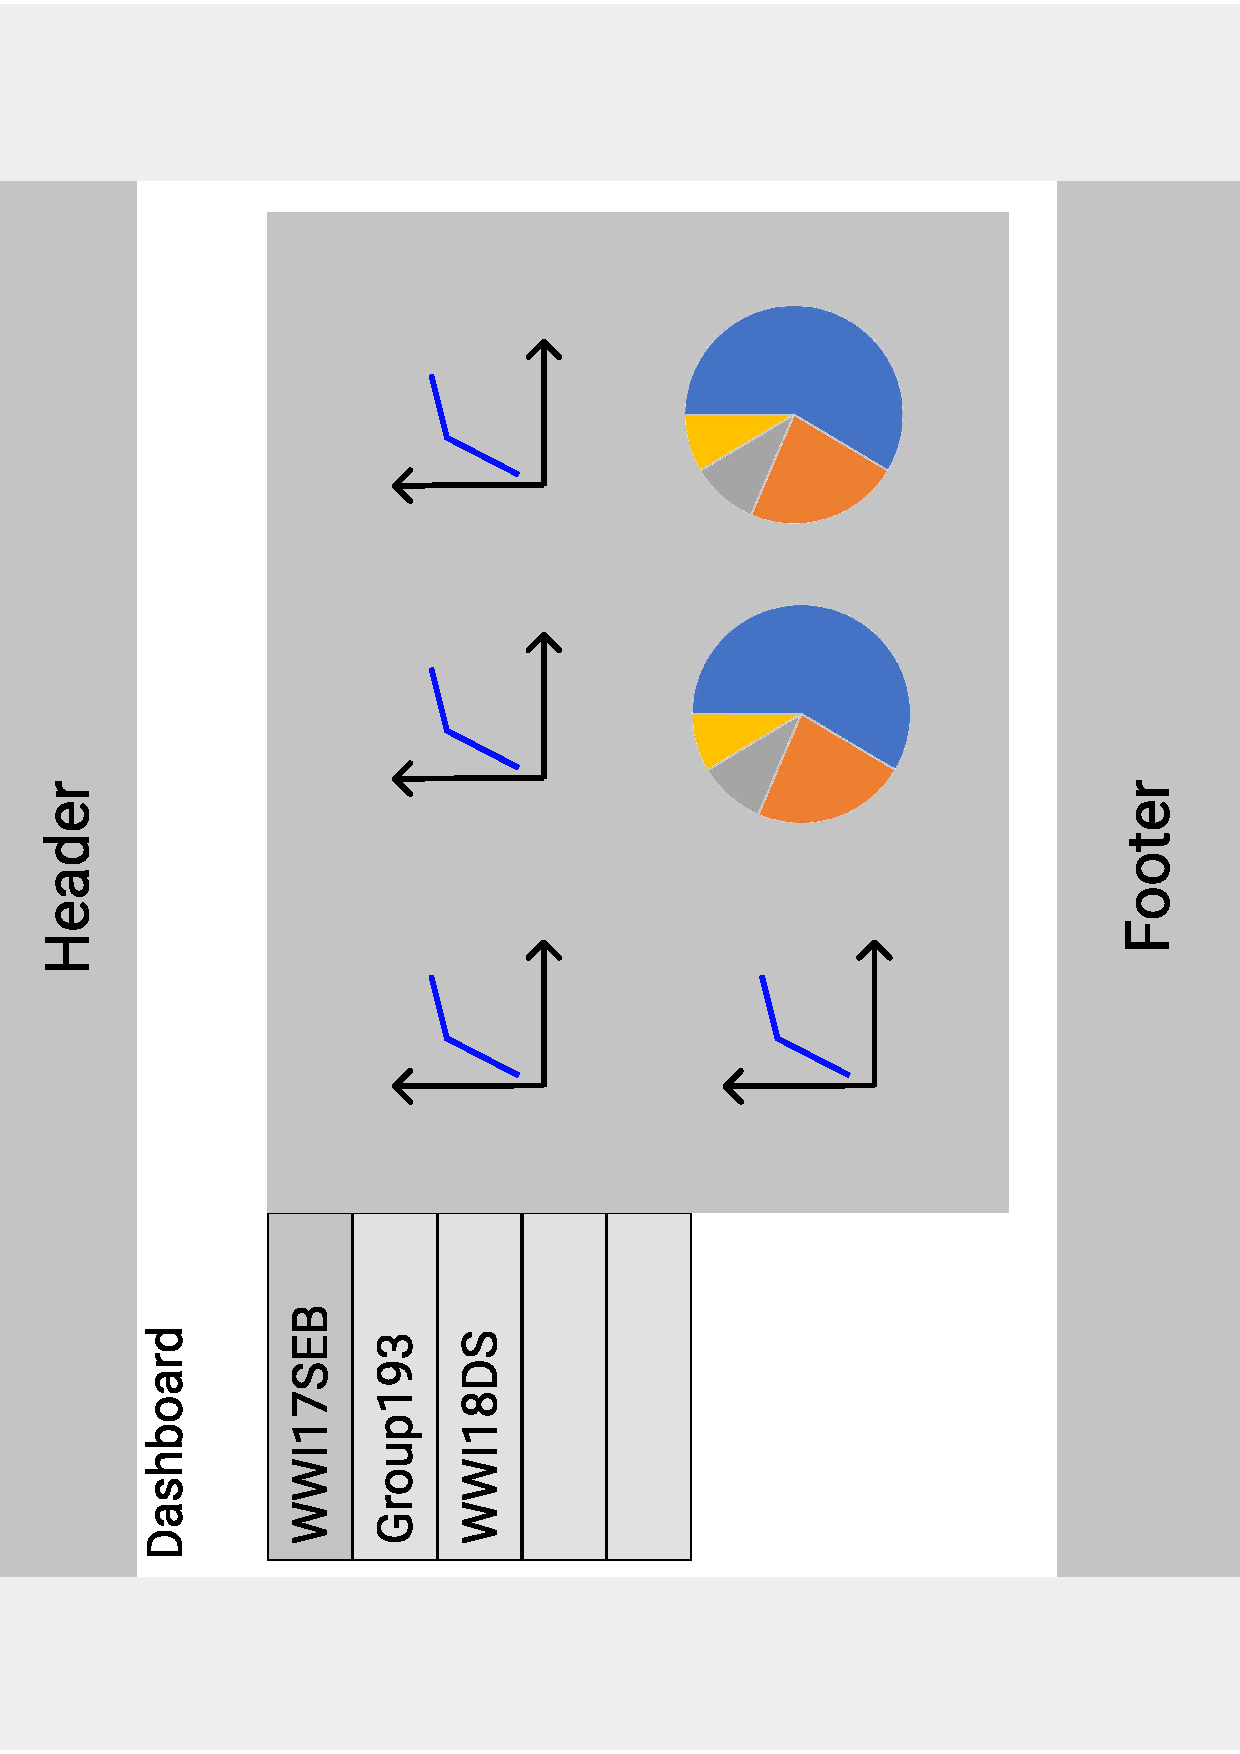
\includegraphics[width=0.7\textwidth]{img/konzeption/client/dashboard}
	\captionsetup{justification=centering, format=plain}
	\caption[Mock-Up des Dashboards]{Mock-Up des Dashboards \\\figma}
	\label{fig:MockDashboard}
\end{figure}



% !TeX root = ../../../master.tex

\subsection{Umfrage erstellen}
\label{ssec:UmfrageErstellen}

Das Herzstück der Applikation soll das Erstellen einer Umfrage sein.
Hier soll der Benutzer die Möglichkeit haben, eine Umfrage zu erstellen, die verschiedene Fragetypen beinhaltet.
Fragetypen sind exemplarisch:
%
\begin{itemize}
	\item Freitext (Single Input)
	\item Checkbox, Matrix (Multiple Choice)
	\item Radiogroup, Matrix (Single Choice)
	\item Dropdown
	\item Rating (Bewertungsskala)
	\item Boolean (Ja/Nein)
	\item Datepicker (Datumsfelder)
\end{itemize}
%

Die Abbildung~\myRefGeneral{fig:SurveyCreatorImplement} stellt den Umfrageeditor der Anwendung dar.
In diesem kann der Benutzer Umfragen erstellen und editieren.
Der Benutzer gibt der Umfrage einen Titel \engl{title} sowie eine Beschreibung \engl{description}.
Er kann mehrere Seiten anlegen und auch jeder Seite einen eigenen \emph{title} und eine eigene \emph{description} zuteilen. \newline
In der Toolbox (linke Seite) kann der Benutzer die verschiedenen Fragetypen über \emph{Drag \& Drop} auf die ausgewählte Seite schieben.
Hier kann der Benutzer die Frage und mögliche Auswahlmöglichkeiten (bei Single/Multiple Choice) definieren.

\begin{figure}[!htb]
	\centering
	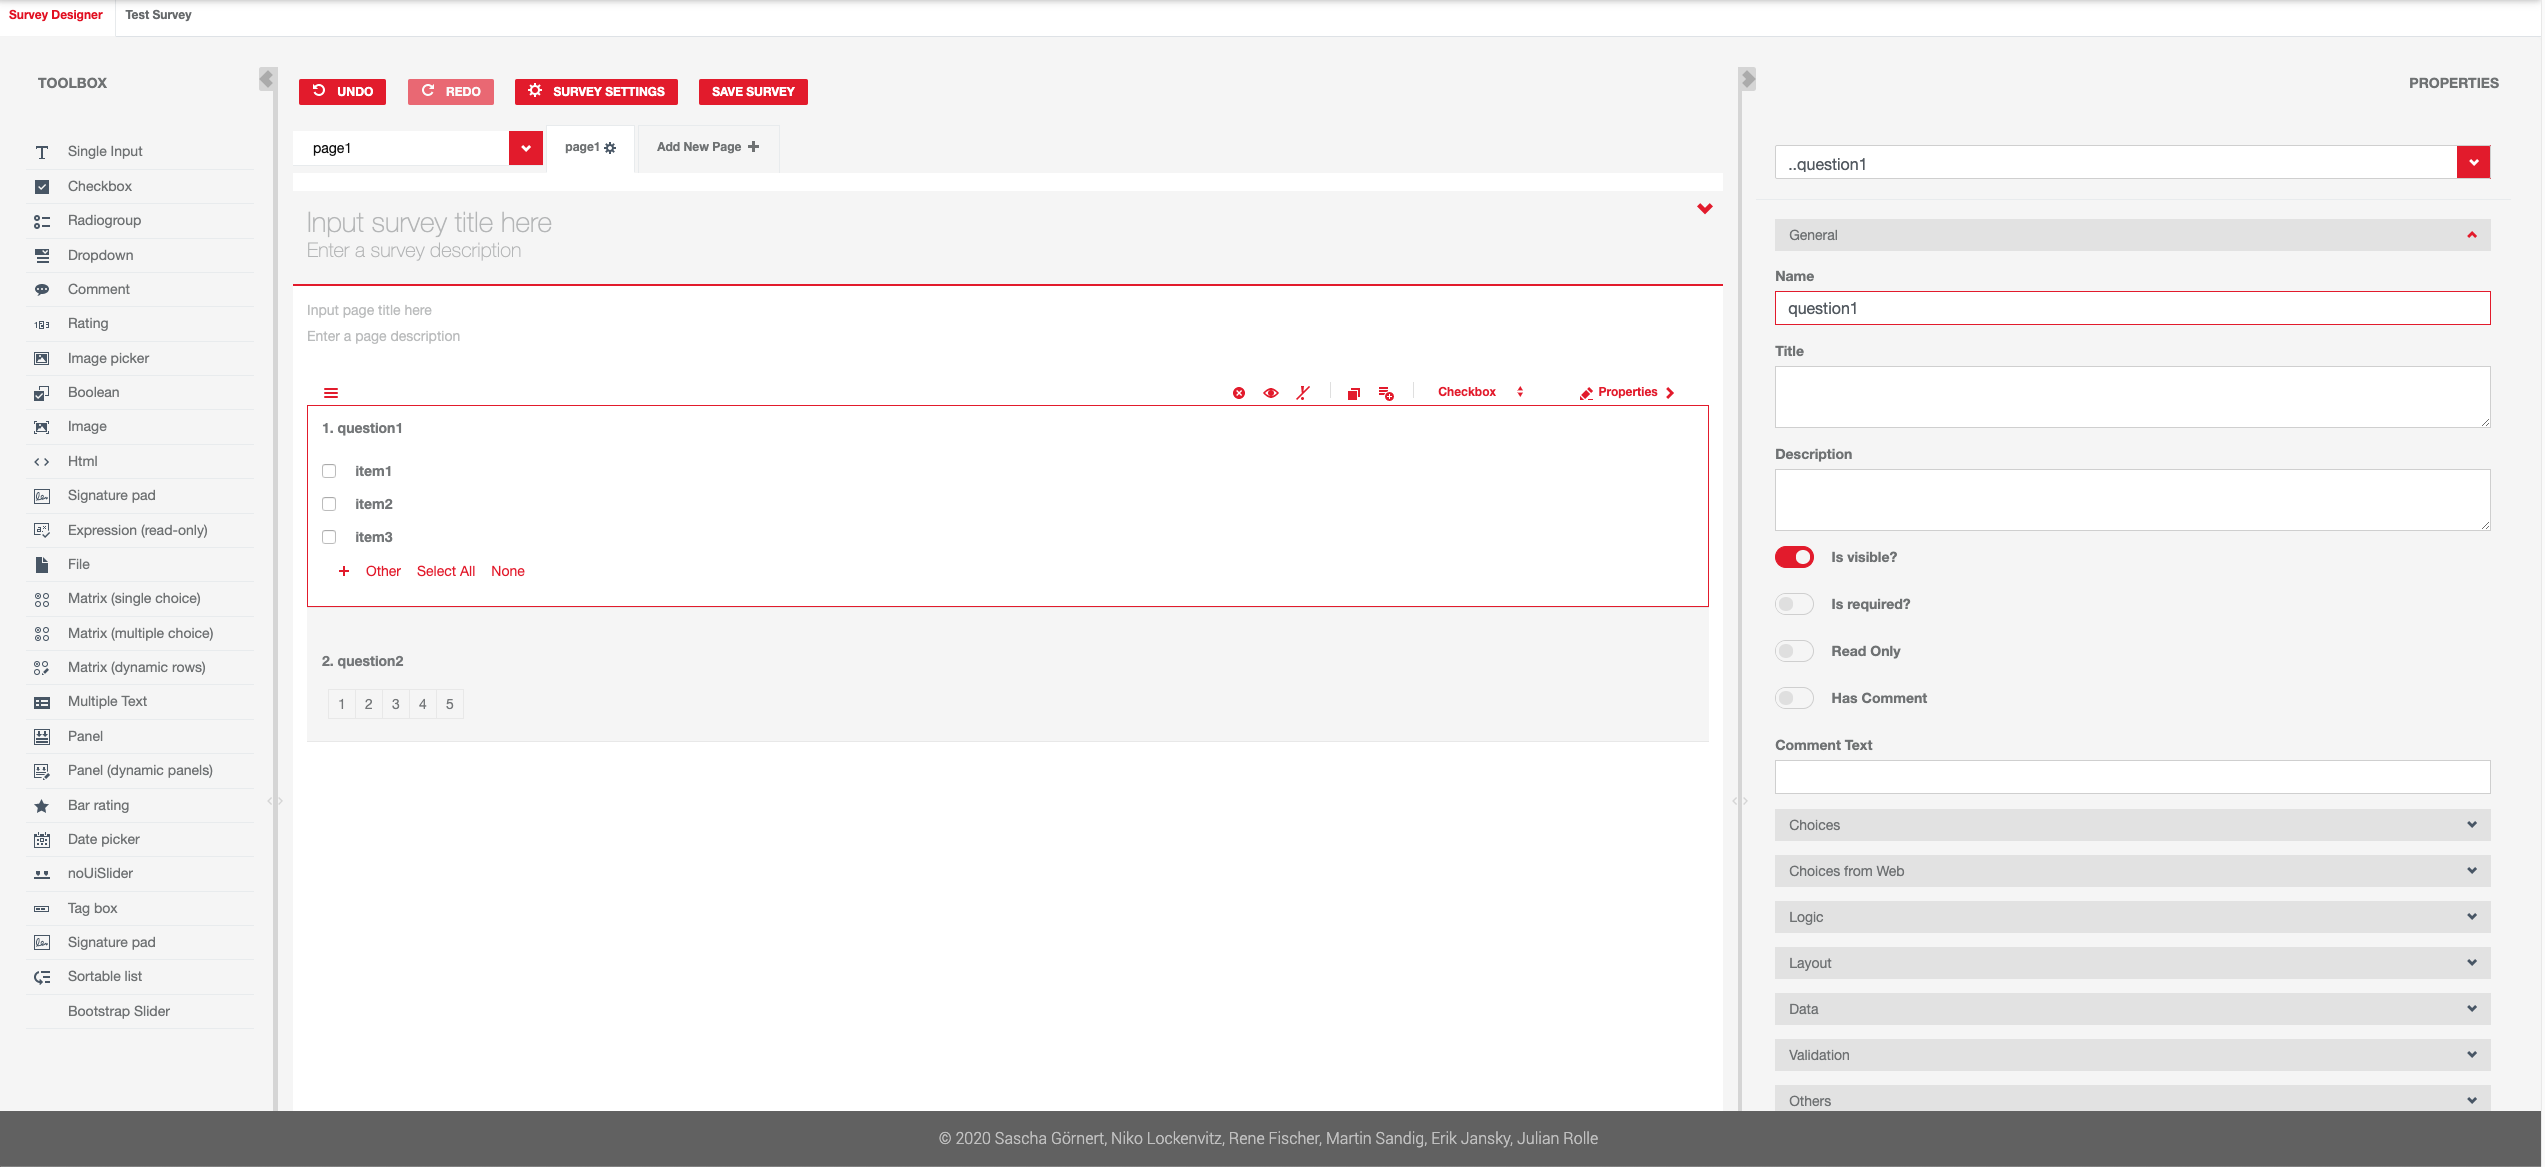
\includegraphics[width=0.95\textwidth, keepaspectratio]{img/client/CreateSurveyMaster.png}
	\captionsetup{justification=centering, format=plain}
	\caption[\acl{UI}: Erstellen einer Umfrage]{\acl{UI}: Erstellen einer Umfrage \\ \quelleScreenshot}
	\label{fig:SurveyCreatorImplement}
\end{figure}

Klickt der Benutzer auf die Schaltfläche \jinline|Test Survey|, werden die erstellten Umfragen dargestellt.
Dabei kann der Nutzer sehen, wie sich die Umfrage auf verschiedene Geräte, wie \zb einem iPhone 8, verhält.
Abbildung~\vref{fig:SurveyAnsicht} zeigt die Möglichkeit, die erstellte Umfrage auf einem bestimmten Gerät \engl{device} zu sehen (hier: Desktop).
Der Benutzer kann die Umfrage über eine Vorschau \engl{preview}, wie in Abbildung~\vref{fig:SurveyMobileAnsicht} dargestellt, auf verschiedenen mobilen Geräten betrachten.
Abbildung~\vref{fig:SurveyMobileAnsichtIPhone8} zeigt die erstellte Umfrage auf einem iPhone 8 an, wohingegen Abbildung~\vref{fig:SurveyMobileAnsichtAndroid} die Umfrage auf einem Android-Smartphone widerspiegelt.

\begin{figure}[!htb]
	\centering
	\captionsetup{justification=centering, format=plain}
	\subfigure[Ansicht der Umfrage]{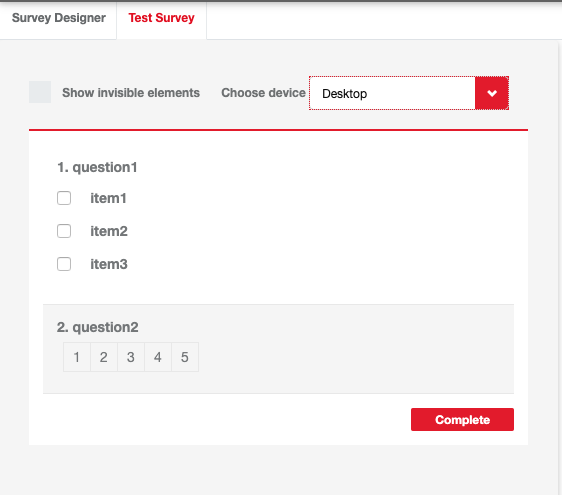
\includegraphics[width=0.48\textwidth]{img/client/CreateSurveyMaster_View1.png}\label{fig:SurveyAnsicht}}\hfill
	\subfigure[Auswahl verschiedener mobiler Ansichten]{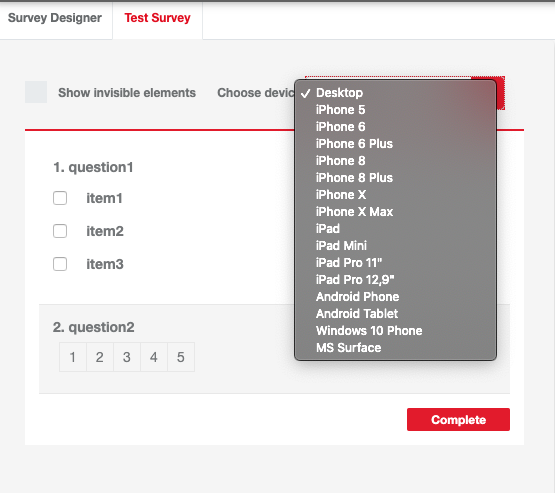
\includegraphics[width=0.48\textwidth]{img/client/CreateSurveyMaster_View2.png}\label{fig:SurveyMobileAnsicht}}\hfill
	\subfigure[Mobile Ansicht: iPhone 8]{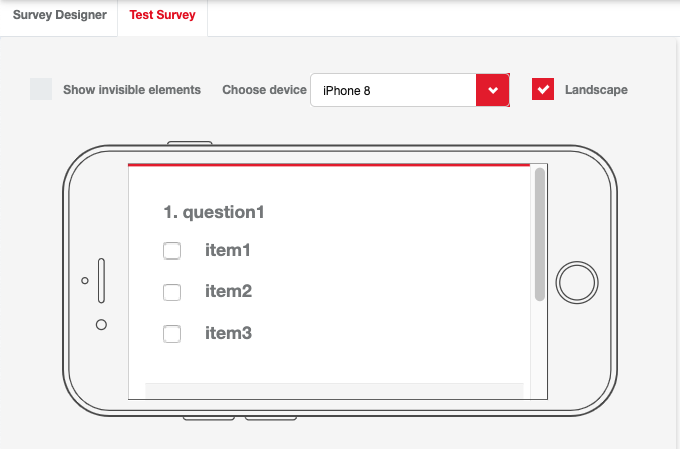
\includegraphics[width=0.48\textwidth]{img/client/CreateSurveyMaster_View3.png}\label{fig:SurveyMobileAnsichtIPhone8}}\hfill
	\subfigure[Mobile Ansicht: Android-Smartphone]{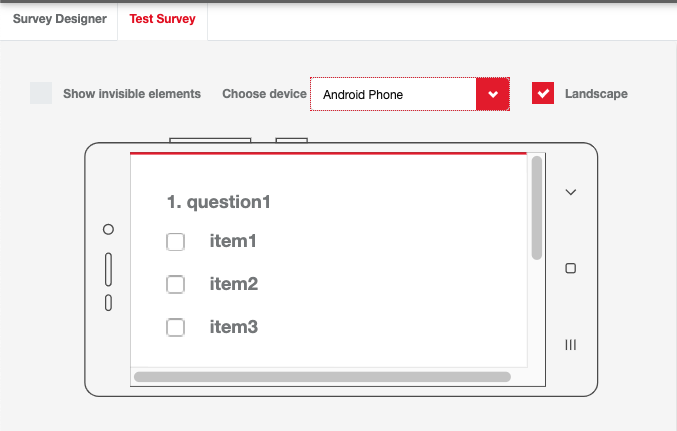
\includegraphics[width=0.48\textwidth]{img/client/CreateSurveyMaster_View4.png}\label{fig:SurveyMobileAnsichtAndroid}}
	\caption[\acl{UI}: Darstellung der erstellten Umfrage auf verschiedenen Geräten]{\label{fig:SurveyCreatorViewImplement}\acl{UI}: Darstellung der erstellten Umfrage auf verschiedenen Geräten \\ \quelleScreenshot}
\end{figure}

Über einen Knopf \jinline|Save Survey| kann der Benutzer die Umfrage speichern.
Zudem erhält der Nutzer ein visuelles Feedback über den Erfolg oder Nichterfolg des Erstellens der Umfrage.
Die erstellten Umfragen erscheinen im \emph{Survey Dashboard} (Kapitel~\vref{ssec:UmfrageDashboard}).


\subsection{Administrationsbereich}
\label{ssec:Administrationsbereich}

Geplant ist, dass die Anwendung einen Administrationsbereich erhält, die es ermöglichen soll: 
\begin{itemize}
    \item Den Registierungsschlüssel einzusehen und zu ändern,
    \item Einen neuen Benutzer anzulegen,
    \item Sowie alle Benutzer in der Anwendung anzuzeigen. 
\end{itemize}

Abb. \myRefGeneral{fig:MockAdministrationsbereich} stellt das Mockup des Administrationsbereich dar. 
Über einen Button soll der Administrator dem Registierungsschlüssel ändern können, sodass im Falle eines \emph{Leaks} des Registierungsschlüssels ein Registrieren eines neuen Benutzers nicht mehr möglich ist. 
Darüber hinaus soll der Administrator ebenfalls neue Benutzer anlegen können sowie alle Benutzer in der Anwendung anzeigen können. 

Hier soll es wie in Abb. \myRefGeneral{MockMakeAdmin} dargestellt wird, soll der Administrator die Möglichkeit haben, das Passwort eines Benutzer neu zu setzen im Falle eines Vergessesens des Benutzers.
Des weitern soll auch ein Benutzer zu einem Administrator upgegraded werden. 

\begin{figure}
	\missingfigure{Administrationsbereich}
	\caption[Mock: Administrationsbereich]{Mock: Administrationsbereich \\ \quelle}
	\label{fig:MockAdministrationsbereich}
\end{figure}

\begin{figure}
	\missingfigure{MockMakeAdmin}
	\caption[Mock: MockMakeAdmin]{Mock: MockMakeAdmin \\ \quelle}
	\label{fig:MockMakeAdmin}
\end{figure}
